%%%%%%%%%%%%%%%%%%%%%%%%%%%%%%%%%%%%%%%%%%%%%%%%%%%%%%%%%%%%%%%%%%%%%%%%%%%%%%%%
%2345678901234567890123456789012345678901234567890123456789012345678901234567890
%        1         2         3         4         5         6         7         8

\documentclass[letterpaper, 12 pt, conference]{ieeeconf}  % Comment this line out
                                                          % if you need a4paper
%\documentclass[a4paper, 10pt, conference]{ieeeconf}      % Use this line for a4
                                                          % paper

\IEEEoverridecommandlockouts                              % This command is only
                                                          % needed if you want to
                                                          % use the \thanks command
\overrideIEEEmargins
% See the \addtolength command later in the file to balance the column lengths
% on the last page of the document
\setlength{\textfloatsep}{8pt plus 1.0pt minus 2.0pt}
\setlength{\floatsep}{8pt plus 1.0pt minus 2.0pt}
\usepackage[margin=0.6in]{geometry}

%\usepackage[margin=0.5in]{geometry}
\usepackage{times}
\usepackage[usenames,dvips]{color}
\usepackage{amsmath}
\usepackage{amssymb}
\usepackage{amsfonts}
\usepackage{graphicx}
\usepackage{multicol}
\usepackage{hyperref}
\usepackage{verbatim}
\usepackage[tight]{subfigure}
\usepackage{cite}
\usepackage[vlined,linesnumbered,ruled]{algorithm2e}
\usepackage{color}
%\usepackage{smallcaptions}
\usepackage{bm}
\usepackage[tight]{subfigure}
\usepackage{amsfonts,amsmath,amssymb}
\usepackage[tight]{subfigure}
\usepackage{cite}
\usepackage[vlined,linesnumbered,ruled]{algorithm2e}
\usepackage{flushend}
\usepackage{amsmath}
\usepackage{multirow}
\usepackage{hhline}
\usepackage{xspace}
\usepackage{bm}
\usepackage{tabularx}
% For table
\usepackage{multirow}
\usepackage{booktabs} % For rules in tables

\usepackage{stmaryrd}
\usepackage{verbatim}

\def\vec#1{{\bf #1}}
\def\S{{\mathbb{S}}}
\def\S2{{\mathbb{S}^2}}
\def\S3{{\mathbb{S}^3}}
% The following packages can be found on http:\\www.ctan.org
%\usepackage{graphics} % for pdf, bitmapped graphics files
%\usepackage{epsfig} % for postscript graphics files
%\usepackage{mathptmx} % assumes new font selection scheme installed
%\usepackage{times} % assumes new font selection scheme installed
%\usepackage{amsmath} % assumes amsmath package installed
%\usepackage{amssymb}  % assumes amsmath package installed

\title{\LARGE \bf Implementation of a Combinatorial Maximum Concurrent Flow Algorithm
}

\author{Matt Jordan and Jin Pan
}
\begin{document}



\maketitle
\thispagestyle{empty}
\pagestyle{empty}


% Abstract

Maximum Concurrent Flow (MCF) is used in a wide range of optimization problems where one needs to send multiple
commodities concurrently across a network to meet a set of demands. In particular, MCF optimizes the minimum fraction of
the how much any one commodity is satisfied.

Here, we implement Garg's combinatorial MCF algorithm and analyze how various heuristics affect theoretical and
experimental runtime.  We also offer a novel heuristic based on sloppy beta scaling and demonstrate better experimental
runtime.


\section{Introduction}

The multicommodity flow problem requires routing multiple commodities
from their respective sources to their respective sinks along a
directed graph. It also requires that the net flow across all commodities on any
single edge does not exceed the capacity of that edge and that flow is conserved. Multicommodity
flow problems arise in many different contexts where distinct
resources need to be concurrently routed across a network. For example,
multicommodity flow problems are solved when routing across
communication networks or determining routing of goods across a transportation network.

Historically, this problem and its many variants have been solved by
formulating the problem as a large linear program \cite{goldberg}. This allows us to
use the multitude of linear programming
algorithms to solve this problem exactly in polynomial time. The
structure of this problem has been used to modify
interior point methods to generate faster runtimes in practice, but
the size of the linear program quickly gets prohibitively large. In
practice, fully polynomial approximation schemes can very closely
approximate a solution to the multicommodity flow problem, even for
large problem instances. In practice, getting within $1\%$ or even
$5\%$ of the optimal solution is often good enough, and can be
attained much more quickly than with linear
programming methods. These fully polynomial approximation schemes
often rely on subroutines which can be efficiently computed in
practice, such as minimum cost flow or single-source shortest paths.

In this paper, we implement an algorithm for solving multicommodity
flow variants first introduced by Garg in 2007 \cite{garg}. 
In particular, we offer
an implementation solving the maximum concurrent flow problem. We also
implement several heuristics that take advantage of certain features
of a problem instance to further speed up the algorithm in
practice. The paper is organized as follows. In section 2
we formally present the problem and define maximum concurrent flow in
addition to discussing previous contributions towards creating an
efficient fully polynomial approximation scheme for this problem. In
section 3, we present the algorithm and offer a brief analysis of its
runtime and correctness. In section 4, we present several heuristics
implemented to speed up runtime in practice. Section 5 contains our
description of our implementation, experiments, results and
discussion.  Finally we offer our concluding remarks in section 6.


\section{Background}
We formally introduce the problem of maximum concurrent flow. We
start with a directed graph $G(V,E)$ with edge capacities 
$c: e \rightarrow \mathbb{R}^+$,
 and $k$ commodities with source $s_j$ and sink $t_j$ for
commodity $j$. Each commodity also has an associated demand
$d(j)$. The problem of maximum concurrent flow is to find a feasible
flow that maximizes the minimal ratio of flow sent to commodity $j$ to the
demand of commodity $j$, over all commodities. Formally, maximum
concurrent flow finds a flow $f$ that maximizes $\lambda$, where for a given flow $f$ that routes $f_j$
units of commodity $j$ from $s_j$ to $t_j$, 
$$\lambda = \min_{j}(f_j/d(j))$$

We remember that a feasible flow preserves capacity constraints: 
$$\sum_j f_j(u,v) \leq c(u,v)$$
where $f_j(u,v)$ represents the flow of commodity $j$ through edge
$(u,v)$ for each edge $((u,v))\in E$, and maintains flow conservation:
$$\sum_{v\in V} f_j(u,v)=0$$ 
for $v\neq s_j,t_j$, for all commodities $j$ and defining
$f_j(u,v)=-f_j(v,u)$. Intuitively, we can describe the maximum
concurrent flow problem as the following situation: we want to send
commodities to their respective sinks, but instead of shooting for the
bare minimum of demand satisfaction, we want to maximize the ratio of
supply to demand for all commodities. This differs from other
multicommodity flow variants, such as the maximum multi-commodity flow
problem where the goal is to simply maximize total throughput from
sources to sinks with no demands on each commodity. Maximizing the minimum ratio is often more desirable in practice,
as this ensures that all commodities that can be filled will be at least partially filled.

Typically the problem of maximum concurrent flow is formulated under the context of a linear
program. If we let $\mathcal{F}_j$ be the set of flows that send $d(j)$ units
of commodity j from $s_j$ to $t_j$, letting
 $\mathcal{F}=\cup_{j=1}^k \mathcal{F}_j$, the set of flows that route
$d(j)$ units of flow from $s_j$ to $t_j$ for any fixed $j$. We can
formulate a linear program with a variable $x(f)$ for each element
$f\in \mathcal{F}$ as follows:
\begin{align*}
\text{max     } \lambda \\
\text{s.t. }\sum_{f\in \cal{F}}f_e\cdot x(f) \leq c(e) \;\;\forall\;
e\in E \\
\sum_{f\in \cal{F}_j} x(f)\geq \lambda \;\;\;\forall\; 1\leq j\leq k \\
x\geq 0,\; \lambda\geq 0.
\end{align*}
Where $f_e$ is defined as the amount of flow that $f$ sends across edge $e$. In this case, $x(f)$ is defined as the fractional amount of times we use the
primitive flow $f$, sending $d(j)$ units of commodity $j$ from $s_j$
to $t_j$ for some $j$. Decoded, the first constraint maintains that no
edge has flow exceeding its capacity. For a particular $j$, the second
constraint ensures that we send more than $\lambda d(j)$ flow to
$t_j$. 

Alternatively, we can model this problem with a
different LP formulation, operating on paths instead of flows. Let
$\mathcal{P}_j$ be the set of paths starting at $s_j$ and ending at
$t_J$.
Then we can define $\mathcal{P}$ to be the union of $\mathcal{P}_j$
for all $j$, that is, $\mathcal{P}$ is the set of all paths from $s_j$
to $t_j$ for any $j$. Let $\mathcal{P}_e$ be the set of paths in
$\mathcal{P}$ such that edge $e$ is in the path. Then our LP
formulation assigns a variable $x(p)$ for each path $p\in \mathcal{P}$
and has the following description:
\begin{align*}
\text{max     } \lambda \\
\text{s.t. }\sum_{p\in \mathcal{P}_e}x(p) \leq c(e) \;\;\forall\;
e\in E \\
\sum_{p\in \mathcal{P}_j} x(p)\geq \lambda\cdot d(j) \;\;\;\forall \;1\leq j\leq k \\
x\geq 0,\; \lambda\geq 0.
\end{align*}
In this case, $x(p)$ can be defined as the amount of flow we send
along path $p$. Then the first set of constraints ensures we don't
send flow across an edge that exceeds the edge's capacity. The second
constraint then maintains that the total flow sent from $s_j$ to $t_j$
is greater than $\lambda$ times the demand $d(j)$, ensuring that we
maximize the minimal ratio of flow to demand over all commodities. Both formulations solve an equivalent problem; however
it is clear that both formulations are exponential in the size of the graph. For this
reason many fully polynomial approximation schemes have been
developed. 
The first fully polynomial approximation schemes (FPAS) for solving
multi-commodity flow problems and their variants arose in the early
90's with Leighton et. al \cite{leighton}.
Typically, variants of multi-commodity flow problems have often been
solved with similar techniques. That is, the tricks that tend to work
well for solving one variant of a multi-commodity flow problem can
easily be extended to other multi-commody flow variants. For this
reason, in discussing the background of maximum concurrent flow (MCF),
we will describe the background of min-cost multi-commodity flow
(MCMCF) which has typically been the problem on which most of the
following techniques were first developed. Keep in mind that FPAS'
for MCMCF are easily extensible to MCF, often using the same tricks,
both in theory and to speed up implmentation in
practice.
Theoretically, these algorithms run faster than
interior-point methods for solving LP's, but it was several years
after the development of the theoretical development of
the first FPAS's that an efficient implementation was developed,
attaining a speed two-to-three orders of magnitude faster than
state-of-the-art linear program solvers \cite{goldberg}.
The main idea of how
these early FPAS' work is a rerouting method, generalizing on
fractional packing techniques \cite{karger}.
Initially, the
algorithm finds an initial flow satisfying the demands, but possibly
violating the capacities. Then the algorithm repeatedly
picks a commodity via round-robin fashion and reroutes flow using a
single-commodity minimum-cost flow in the auxiliary graph until the flow is feasible. The costs
on the edges of the auxiliary graph are initialized to a small value,
but are scaled for every unit of flow rerouted through them, ultimately
making the cost of an edge exponential in the amount of flow sent
through it. The 'goodness' of the reroutings are stored in a potential function, which
is guaranteed to generate a $1+\omega$ solution in
$\tilde{O}(\omega^{-3}kmn)$ time for the minimum cost multi-commodity flow
problem \cite{karger}. 
Since then, these bounds have since been increased to
$\tilde{O}(\omega^{-2}m^2)$ in 2000 \cite{grig}. 
Most recently, Jonathon Kelner of MIT proposed a method to find an $\omega$ approximate concurrent multicommodity flow problem
in  $O(m^{1+o(1)}\omega^{-2}k^2)$ time
using a combination of a
non-Euclidean generalization of gradient descent, flow sparsifiers,
and an $O(m^{o(1)})$-competitive oblivious routing scheme \cite{almostLinear}. 

\section{Algorithm}
\subsection{Presentation of algorithm}
Avoiding the complicated methods of the most recent publication
improving the bounds for maximum concurrent flow, we choose to
implement the maximum concurrent flow FPAS presented by Garg and
K\"{o}nemann and several heuristics to speed up runtime in
practice. The basic implementation gives a runtime of
$\tilde{O}(\omega^{-2}(k+m)m)$ for the MCF problem \cite{garg}. The dependency on $k$
can be removed with
the implementation of our heuristics as described later. For the
remainder of this section, we will describe the algorithm implemented
in this paper (herein referred to as Garg-MCF), offering both
pseudocode and a brief look at the analysis. \\
The main idea behind Garg-MCF relies on the rerouting and fractional
packing methods introduced in section 2. In plain english, we compute
a $(1+\omega)$ approxmation as follows. We start by adjusting the
demands of each commodity such that the optimal solution to the LP is
at least 1; this is done for the sake of the analysis. We proceed by assigning a 'length' to each edge
dependent upon $\omega$ and
the capacity of that edge. We repeatedly satisfy the
demand of each commodity by sending as much flow as we can
(independently) along the
shortest path from the source to the sink, where shortest is dependent
upon the `length' function. Then we scale the `length' of each edge by
a factor dependent upon the amount of flow we just sent across it. In
this way, the `length' is exponential in the amount of flow being sent
across the edge. Intuitively, since we call shortest paths based on
this length function, this causes us to spread our flow across edges
and reroute in such a fashion that doesn't force all our flow on one
path. We rescale the demands as we proceed to speed up runtime, but
also maintain that the optimal $\lambda$ is at least 1. We stop after the length functions grow `large enough'. The
precise definition of `large enough' and that this computes a $1+\omega$ approximation is not
entirely obvious, but is believable under the context of the
analysis. We will be more formal in how Garg-MCF works
now.

Consider the second linear program formulation of maximum
concurrent flow, which we will refer to as P-MCF. Taking the dual of
P-MCF generates the following linear program, which we'll refer to as D-MCF, which defines a length
$l(e)$ for each edge and a variable $z(j)$ for each commodity.
\begin{align*}
\text{min     } \sum_{e\in E}c(e)l(e) \\
\text{s.t. }\sum_{e\in p}l(e) \geq z(j) \;\;\forall 1\leq j \leq k,
\forall p \in \cal{P}_j\\
\sum_{j=1}^kd(j)\cdot z(j)\geq 1\\
l,z\geq 0
\end{align*}
Recalling that $\mathcal{P}_j$ is the set of paths from $s_j$ to
$t_j$. Intuitively, the first constraint maintains that, when tight, $z(j)$ is the
value of the length of the shortest path from $s_j$ to $t_j$. Keeping
with Garg's notation, we define the objective value to be a function
of the length assignment $l$:
$$D(l) := \sum_{e\in E} c(e)l(e)$$
and define $\alpha(l)$ as the second constraint, also a function of the length assignment $l$:
$$\alpha(l) := \sum_{j=1}^k d(j)\cdot z(j)$$

Then since we'll have a minimal objective value when the second
constraint is tight, this LP can be viewed as the assignment of
positive lengths to edges such that $\frac{D(l)}{\alpha(l)}$ is
minimized. 

With notation in hand, the algorithm runs as follows. We first scale
the demands of each commodity in a fashion to ensure that the optimal
value is at least 1. This scaling factor is referred to as
$\frac{k}{z}$ with the derivation shown in the original paper. The exact mechanism by which this is done isn't
as important as noticing that scaling the demands by a constant factor
scales the value of $\lambda$ by the inverse of that constant
factor. Next, we assign
an initial length of $\delta/c(e)$ to each edge, where $\delta$ is carefully picked
to make the analysis work out. Then we proceed in phases. For each
phase, we loop through each commodity $j$ in a series of $k$
iterations, one for each commodity. For each $j^{th}$ iteration then, we
consider commodity $j$ and reroute $d(j)$ units of flow from $s_j$ to
$t_j$. We do this with a series of steps, updating the length after each step. Let $l_{i,j}^s$ refer to the
length function at the $i^{th}$ phase, the $j^{th}$ iteration,
directly after the $s^{th}$ step. Then during each step, we compute the minimum cost
path from $s_j$ to $t_j$ under this length function, $l_{i,j}^s$, and route as much
flow along that path as possible. That is, we wish to route a total of
$d(j)$ flow from $s_j$ to $t_j$ over all steps during an iteration, so
let $d^s$ refer to flow remaining to be rerouted during an
iteration, after $s$ steps. Initially $d^0=d(j)$ and conclude the
iteration when $d^q=0$ for some $q$. 

Then for each step, we compute a path $p$,
and we route $f_{i,j}^{s+1}$ flow along this path, where
$f_{i,j}^{s+1}$ is the maximum allowable flow we can send, or in other
words, the minimum between the capacity of the minimum capacity edge
in $p$ and the flow remaining to be sent during this iteration. So
$$f_{i,j}^{s+1}=\min(\min_{e\in p}(c(e)),d_{i,j}^s)$$
We then decrease the amount of flow remaining to be routed, $d^s$ by
$f_{i,j}^{s+1}$. Since we routed flow along every edge in $p$, we also
need to update the length function for these edges, so we do this by
multiplying $l_{i,j}^s(e)$ by $1+\epsilon \frac{f_{i,j}^{s+1}}{c(e)}$ for an
$\epsilon$ that we define later, dependent upon $\omega$. 

We terminate
the iteration when $d_{i,j}^p=0$ for some step number $p$. We repeat
this process for each commodity during an iteration, and we repeat
phases until we reach our stopping condition, which we define when 
$D(l_{i,j}^s)\geq 1$, which is checked at the end of every
phase. Also, upon completion of a certain number of phases, $T$, we can
guarantee that the optimal value is greater than 2, so we can rescale
the demands of each commodity by a factor of 2, and we maintain the
invariant that the optimal value is at least 1. 
Upon completion of the algorithm, we have a graph that has flow along edges, but
almost surely overflows capacity bounds. We can scale the flow along each edge by
dividing flow by $\log_{1+\epsilon}\delta^{-1}$, which makes the
flow feasible. From here, we can calculate $\lambda$
directly. Motivation for calculation of $\delta$, $\epsilon$, and the
final scale factor, $\log_{1+\epsilon}\delta^{-1}$, will be
briefly described in the next section, and fully derived in the
original paper. 
For clarity, we present the pseudocode of this
algorithm in Algorithm 1.

\SetAlgoSkip{}
%%%%%%%%%%%%%%%%%%%%%%%%%%%%%%%%%%%%%%%%%%%%%%%%%%%%%%%%%%%%%%%%%%%%%%%%%%%%%%%%%%%%%%%%%%
\begin{algorithm}[H] \small
$G \leftarrow (V,E)$\;
$\epsilon,\delta \leftarrow \mathrm{calculate\_epsilon}(\omega),\mathrm{calculate\_delta}(\omega)$\;
\For{ $e \in E$}{
  $l(e)=\delta / c(e)$\;
}
$\mathrm{scale\_demands}(\frac{k}{z})$\;
$phase\_since\_rescale \leftarrow 0$\;
\While{$D(l)<1$}{
  \If{ $phase\_since\_rescale>T$}{
  $\mathrm{scale\_demands}(2)$\;
  $phase\_since\_rescale \leftarrow 0$\;
}
  \For{ $j = 1$ to $k$}{
    $d_j \leftarrow d(j)$\;
    \While{$d_j \neq 0$} {
      $p \leftarrow \mathrm{shortest\_path(s_j,t_j)}$\;
      $min\_cap \leftarrow \infty$\;
      \For{$e\in p$}{
        $min\_cap \leftarrow \min(c(e),min\_cap)$\;
      }
      $f \leftarrow \min(min\_capacity,d_j)$\;
      $d_j \leftarrow d_j - f$\;
      \For{$e \in p$}{
        $e.flow \leftarrow e.flow+f$\;
        $l(e) \leftarrow l(e) \cdot (1+\epsilon \cdot f / c(e))$\;
        }

      }
    }
    $phase\_since\_rescale +=1$\;
}
$scale\_factor \leftarrow \log_{1+\epsilon}\delta^{-1}$\;
\For{$e\in E$}{
  $e.flow = e.flow / scale\_factor$\;
  }

\Return{$\mathrm{calculate\_lambda(G)}$}\;
\caption{GARG-MCF without heuristics}
\end{algorithm}
%
% Restore default vertical spacing
\SetAlgoSkip{smallskip}


\section{Analysis}
We offer a brief, high-level overview of the analysis. We point the
reader to the original paper for a more in-depth analysis.
\subsection{Approximation Ratio}
To prove the correctness of Garg-MCF, we care about approximating a
feasible solution to the dual LP, D-MCF. The key idea here is to compare
our calculated $\lambda$ value to the best-possible solution to the
dual LP, D-MCF. Bounding this ratio above by $(1+\omega)$ will attain
the appropriate approximation ratio, since the ratio is bounded below
by 1, according to weak duality. We'll briefly sketch how this is
done below.

We first assume that the
optimal objective value, $\beta$, will be at least 1. We can remove this
assumption later. Then we notice a relation between the objective
value at phase $i$ and phase $i-1$ and use this to establish a bound
on the optimal objective value divided by the number of phases we must
run through to reach our stopping condition. We next can create a
lower bound for $\lambda$ using the knowledge of how much flow we must
route through each edge up to the penultimate phase. It is here that
our scaling factor is derived, and a lower bound for $\lambda$
established dependent on the number of phases completed and
$\epsilon$. 

Now we can consider the ratio between $\beta$ and $\lambda$, since we have bounds on both terms. If we can show that
$\beta/\lambda\leq \text{poly}(\epsilon)$ then by weak duality we have
that $\lambda \leq \beta$, so our computed $\lambda$ is within a
factor of $\text{poly}(\epsilon)$ of $\beta$. Strong duality implies
that $\beta$ is the value of the optimal solution to MCF. With the
math of the paper  we arrive at the claim that 
$$\frac{\beta}{\lambda}\leq (1-\epsilon)^{-3}$$
Thus, if we choose $\epsilon$ such that 
$$(1-\epsilon)^{-3}\leq 1+\omega$$ 
we arrive at our desired $1+\omega$ approximation.
\subsection{Scaling Beta}
We now lift the previous assumption that $\beta\geq 1$. The key idea
here is that by scaling all the demands by a constant factor, we also
scale the value of $\lambda$, and therefore $\beta$. We
find bounds above and below for $\beta$ based on the current demand
scheme, and then scale the demands such that the lower bound for
$\beta$ is 1. It turns out that for any phase number $i$ in which the
algorithm has not yet terminated, $i$ is strictly less than
$\frac{\beta}{\epsilon}\log_{1+\epsilon}\frac{m}{1-\epsilon}$. Then we
can run phases until we have computed enough
phases to ensure that $\beta\geq 2$, a number we'll call $T$. In this case
we scale demands of
all commodities, effectively reducing $\beta$ by a factor of
two. If the ratio of the upper bound and lower bound for $\beta$ was
initially $c$, then we have to run for at most $T\log c$ phases. In
the full proof, Garg showed that $c=m$, so we have to run for at most
$T\log m$ phases.
\subsection{Running time}


The scaling of $\beta$ gives us a bound on the number of phases we
must compute. Since we compute $k$ iterations per phase, this also
bounds the number of iterations we must complete. To compute runtime,
we need to calculate the total number of steps we can perform. The key
insight here is that there are two different types of steps: steps
where we saturate an edge, and steps that do not. Notice that in each
iteration, all steps saturate an edge, except the last step in the
iteration. This is to say that for all but the last iteration, at
least one edge has a length that is scaled by a factor of
$1+\epsilon$. Also note that $l(e)c(e)$ is $\delta$ for each edge $e$
initially, and no
more than $1+\epsilon$ at termination, since we terminate as soon as
$\sum_el(e)c(e)\geq 1$ and we scale each edge by no more than
$1+\epsilon$ each time we scale. Thus, the total number of saturating
steps is $m\log_{1+\epsilon}\delta^{-1}$. By setting $\delta$ to
$(m/(1-\epsilon))^{-1/\epsilon}$, the number of saturating steps is at most
$\frac{m}{\epsilon}\log_{1+\epsilon}\frac{m}{1-\epsilon}$. Since the
total number of steps is the number of saturating steps plus the
number of non-saturating steps, and the number of non-saturating steps
is equivalent to the number of iterations, we have that the total
number of steps is no more than 
$T\log m+\frac{m}{\epsilon}\log_{1+\epsilon}\frac{m}{1-\epsilon}$. For
appropriate choice of $\epsilon$ we combine these to show that we get
a runtime of $(\omega^{-2}(k\log m+m)\log m)T_{sp})$ where $T_{sp}$ is the time to
compute a single-source shortest path subroutine.


\section{Heuristics}
In this section we present two  previously developed heuristics and
one novel heuristic that reduces the number of phases or shortest
path computations in practice, in addition to affecting the
theoretical runtime.
\subsection{2-approximation for Beta estimation}
This heuristic allows us to greatly reduce the number of phases we
perform by bounding $\beta$ between 1 and 2. To do this, we first
compute a 2-approximation to the problem using $O(\log k \log m)$
phases, and returns a $\hat{\beta}$ such that $\beta\leq \hat{\beta}\leq2\beta$. Then we don't have to scale demands using the above procedure
and reduces the number of phases to $O(\log m(\log
k+\epsilon^{-1}))$.%CHECK THIS

\subsection{Karakostas' method for shared sources}
This heuristic allows us to remove the depedence upon $k$, the number
of commodities, using a technique first introduced by Karakostas \cite{karakostas}. 
Since
we compute shortest paths using a single-source shortest path method,
with no additional runtime we obtain the minimum cost path from the
source to all possible sinks. Grouping the commodities by shared
sources, we can run the iterations for every commodity in a particular
group at the same time. To do this we make only one call to Djikstra's
for each group for each step and route a scaled flow along the path
associated with each commodity. We scale each flow for commodity $j$
by the ratio of the demand remaining for commodity $j$ to the sum of
demands remaining for all other commodities within this group. The
above analysis still holds since we scale at least one edge by a
factor of $1+\epsilon$ for each step except the last. The number of
iterations then, is equivalent to the number of groups, which is at most
$n$. Thus our runtime of $O(\omega^{-2}(k\log m+m)\log m T_{sp})$
becomes $O(\omega^{-2}(n\log m+m)\log m T_{sp})$, or $\tilde{O}(w^{-2}m^2)$.
\subsection{Removal of demand-scaling}
This novel heuristic was developed to further simplify the algorithm
and has been shown to provide a slight decrease in runtime in
practice. The key idea here is that we consider whether or not it is
possible for $\beta$ to be less than 1. If so, we do not do any
demand-scaling. Otherwise, we scale demands as outlined in Garg-MCF. We can do this only under
the provision that we do not check the termination condition until the
end of each phase. We offer sketches of proofs that this heuristic can
only improve runtime (in practice), and maintains a $(1+\omega)$
approximation. 


For runtime, we have that the runtime is equivalent to the number of
steps times the time to compute a shortest path. Each step is either a
saturating step, where we send flow such that an edge is saturated, or
it isn't, in which case it is the last step of the iteration. Our
bound on the number of saturating steps remains the same, by the same
arguments presented in the above analysis. The number of unsaturating
steps, however, depends on the number of phases, and therefore on the
scaling of demands. Suppose that demand-scaling causes demands to
decrease. Then each iteration routes less flow through, and since the total
flow pushed through the graph upon termination is not dependent upon
the scaling factor, this increases the number of non-saturating steps
we have to perform. In other words, this scaling increases the number
of iterations and therefore the runtime. If demand-scaling causes
demands to increase, then by not doing demand scaling, we lose out on
potential improvement, so we still scale demands in this case. Thus,
we offer no changes to theoretical runtime, but show a runtime
improvement in practice.

It should be noted that the analysis presented by Garg assumed that
$\beta\geq 1$, and this constraint is loosened by not scaling
demands. We claim that, given an adjustment of the flow-scaling factor
applied upon termination, we maintain a $(1+\omega)$
approximation. Note that we only check the termination condition at
the end of every phase. This implies that the ratios of flow sent for
each commodity are constant (i.e., we send $d(j)$ flow of commodity
$j$ for each phase if we don't scale, and $cd(j)$ flow of
commodity $j$ each phase when we do scale, for scaling factor
$c$). Thus we do not artificially increase the objective value by
sending more flow to any one commodity, relative to the demand of that
commodity. However, this relaxation breaks the analysis presented in
Garg claiming that the flow-scaling factor returns the generated flow
to feasibility. We remedy this by noting that the ratios of flow sent
through a commodity to their demand is constant, and thus by
not-scaling demands, we maintain the appropriate ratios of flows for a
$(1+\omega)$ approximation. We return this flow to feasibility by
simply finding the maximum overloaded edge $m$, and scaling the flow
across all edges by the ratio of $c(m)$ to the flow through $m$. 

\section{Experimental Results}

We have implemented Garg-MCF in the Python programming language and
have tested it upon a variety of problems. Due to the automatic
garbage collection of Python, clock time of the implementation should
be taken with a grain of salt. Instead, we measure the number of calls
to the single-source shortest path subroutine. Since we make one call
per step this serves as a valid measurement of runtime. We first
describe the construction of random graphs. \\
We construct random directed graphs using the networkx module's
$\mathrm{gnm\_random\_graph}$ routine, feeding parameters of $n$ and
$m$. Then we randomly create commodities by a grouping
procedure. We take the number of commodities as a parameter and a
distribution which defines the number of shared source commodities we
have, randomly choosing sinks for the commodities, ensuring that there
exists a directed path from the source to the sink for each
commodity. Capacities and demands are chosen randomly. This set of
procedures allows us to randomly generate a directed graph with a
given number of nodes, edges, commodities, and we can explicitly specify the
number of commodity groups. With this in hand, we can proceed to test
the algorithm's dependence on $\omega$ and $k$, taking note of the
effect of Karakosta's heuristic for shared source commodities.
\subsection{Dependence on the parameter $\omega$}

\subsection{Dependence on the parameter $k$}.



\section{Conclusions}

That's all.


\addtolength{\textheight}{-12cm}   % This command serves to balance the column lengths
                                  % on the last page of the document manually. It shortens
                                  % the textheight of the last page by a suitable amount.
                                  % This command does not take effect until the next page
                                  % so it should come on the page before the last. Make
                                  % sure that you do not shorten the textheight too much.

%%%%%%%%%%%%%%%%%%%%%%%%%%%%%%%%%%%%%%%%%%%%%%%%%%%%%%%%%%%%%%%%%%%%%%%%%%%%%%%%



%%%%%%%%%%%%%%%%%%%%%%%%%%%%%%%%%%%%%%%%%%%%%%%%%%%%%%%%%%%%%%%%%%%%%%%%%%%%%%%%



%%%%%%%%%%%%%%%%%%%%%%%%%%%%%%%%%%%%%%%%%%%%%%%%%%%%%%%%%%%%%%%%%%%%%%%%%%%%%%%%
%Appendixes should appear before the acknowledgment.

%\section*{ACKNOWLEDGMENT}
%The preferred spelling of the word ÒacknowledgmentÓ in America is without an ÒeÓ after the ÒgÓ. Avoid the stilted expression, ÒOne of us (R. B. G.) thanks . . .Ó  Instead, try ÒR. B. G. thanksÓ. Put sponsor acknowledgments in the unnumbered footnote on the first page.



%%%%%%%%%%%%%%%%%%%%%%%%%%%%%%%%%%%%%%%%%%%%%%%%%%%%%%%%%%%%%%%%%%%%%%%%%%%%%%%%

%References are important to the reader; therefore, each citation must be complete and correct. If at all possible, references should be commonly available publications.





\bibliographystyle{plain}
\bibliography{references}


\begin{figure*}
\begin{center}
\mbox{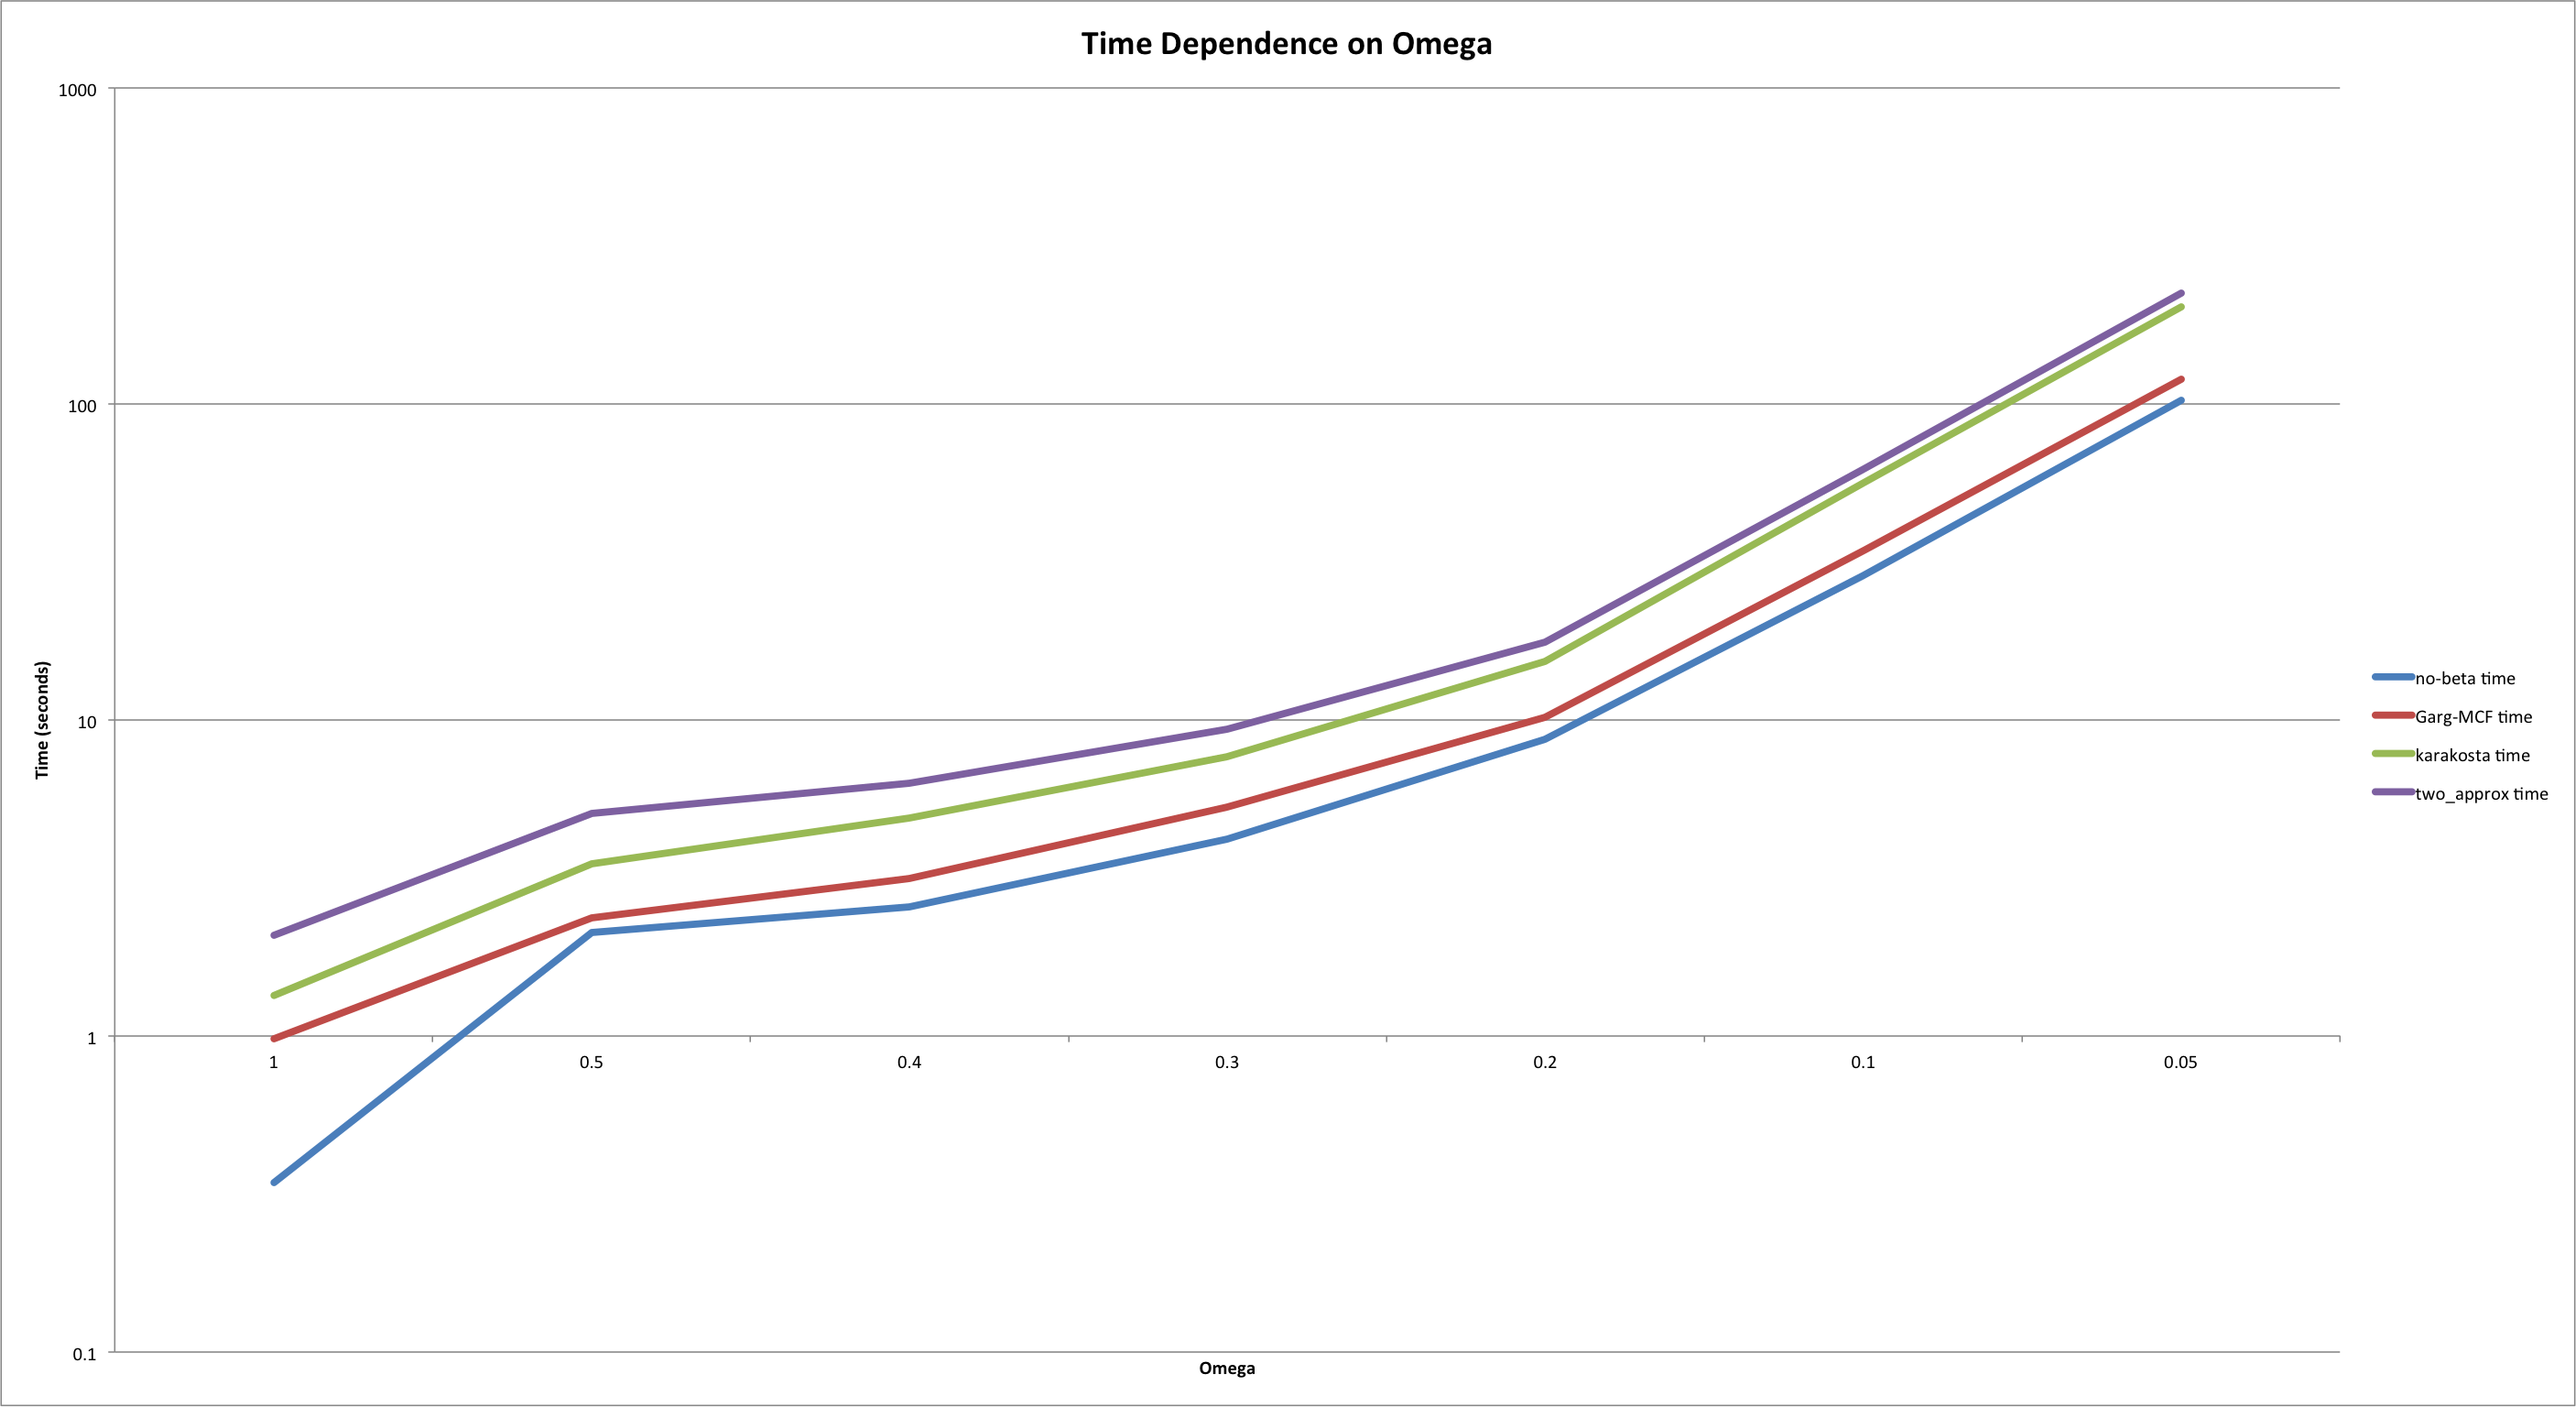
\includegraphics[width=0.8\textwidth]{figures/omegas-time.png}}
\caption{Plots of time in seconds versus error term $\omega$ for all heuristics}
\end{center}
\end{figure*}

\begin{figure*}
\begin{center}
\mbox{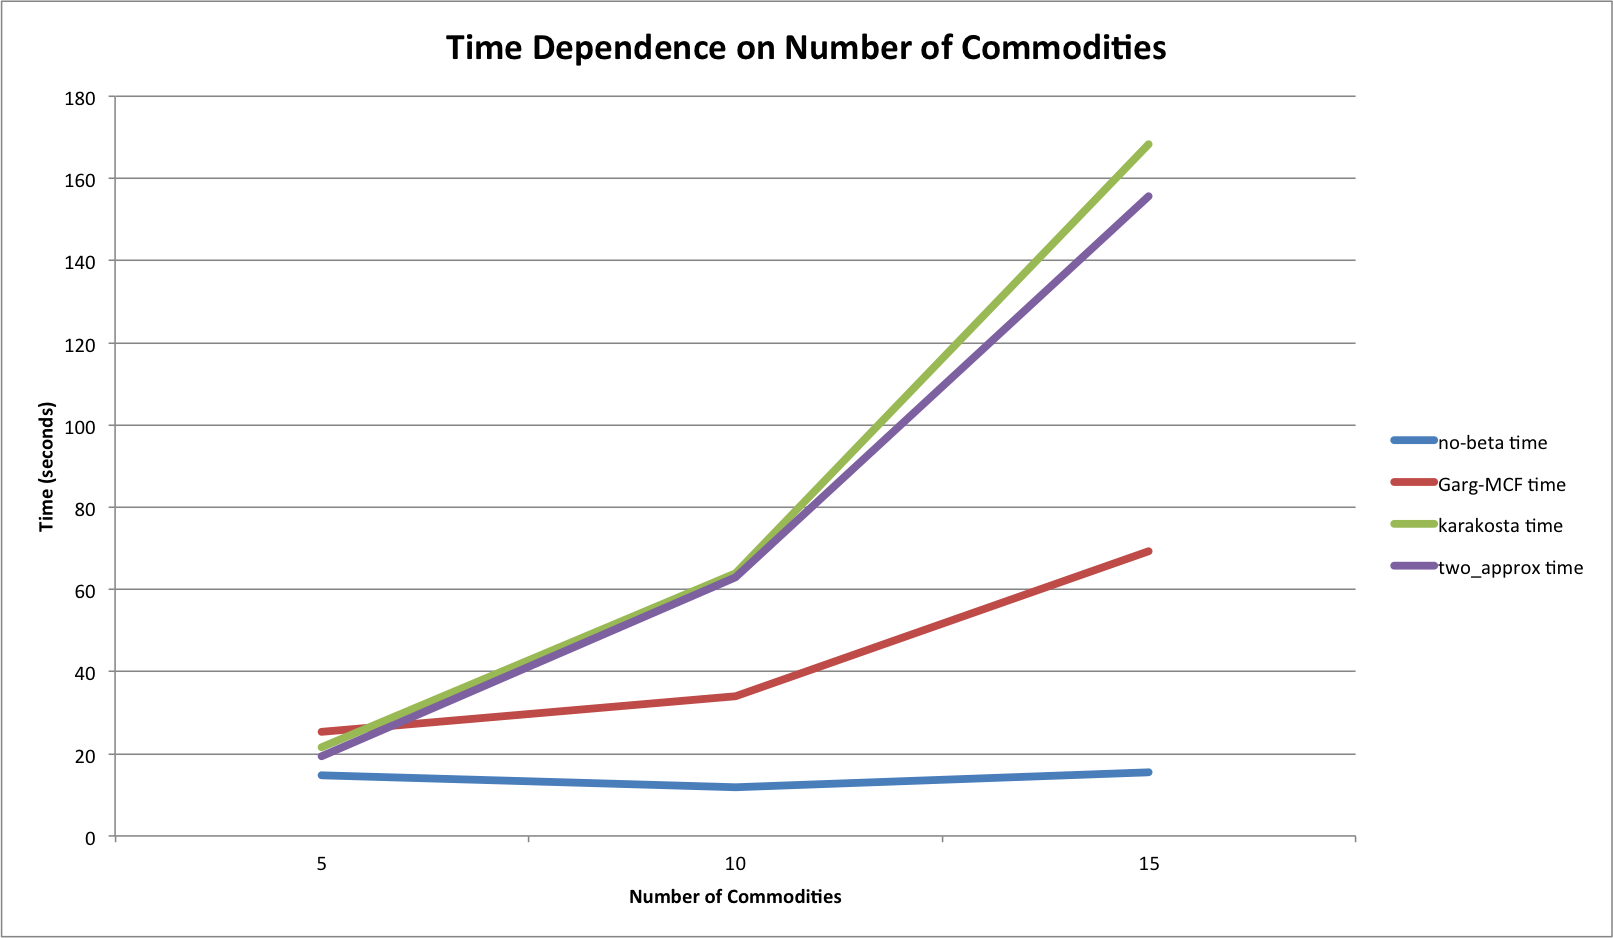
\includegraphics[width=0.8\textwidth]{figures/commodities-time.png}}
\caption{Plots of time in seconds versus number
  of commodities for all heuristics}
\end{center}
\end{figure*}

\begin{figure*}
\begin{center}
\mbox{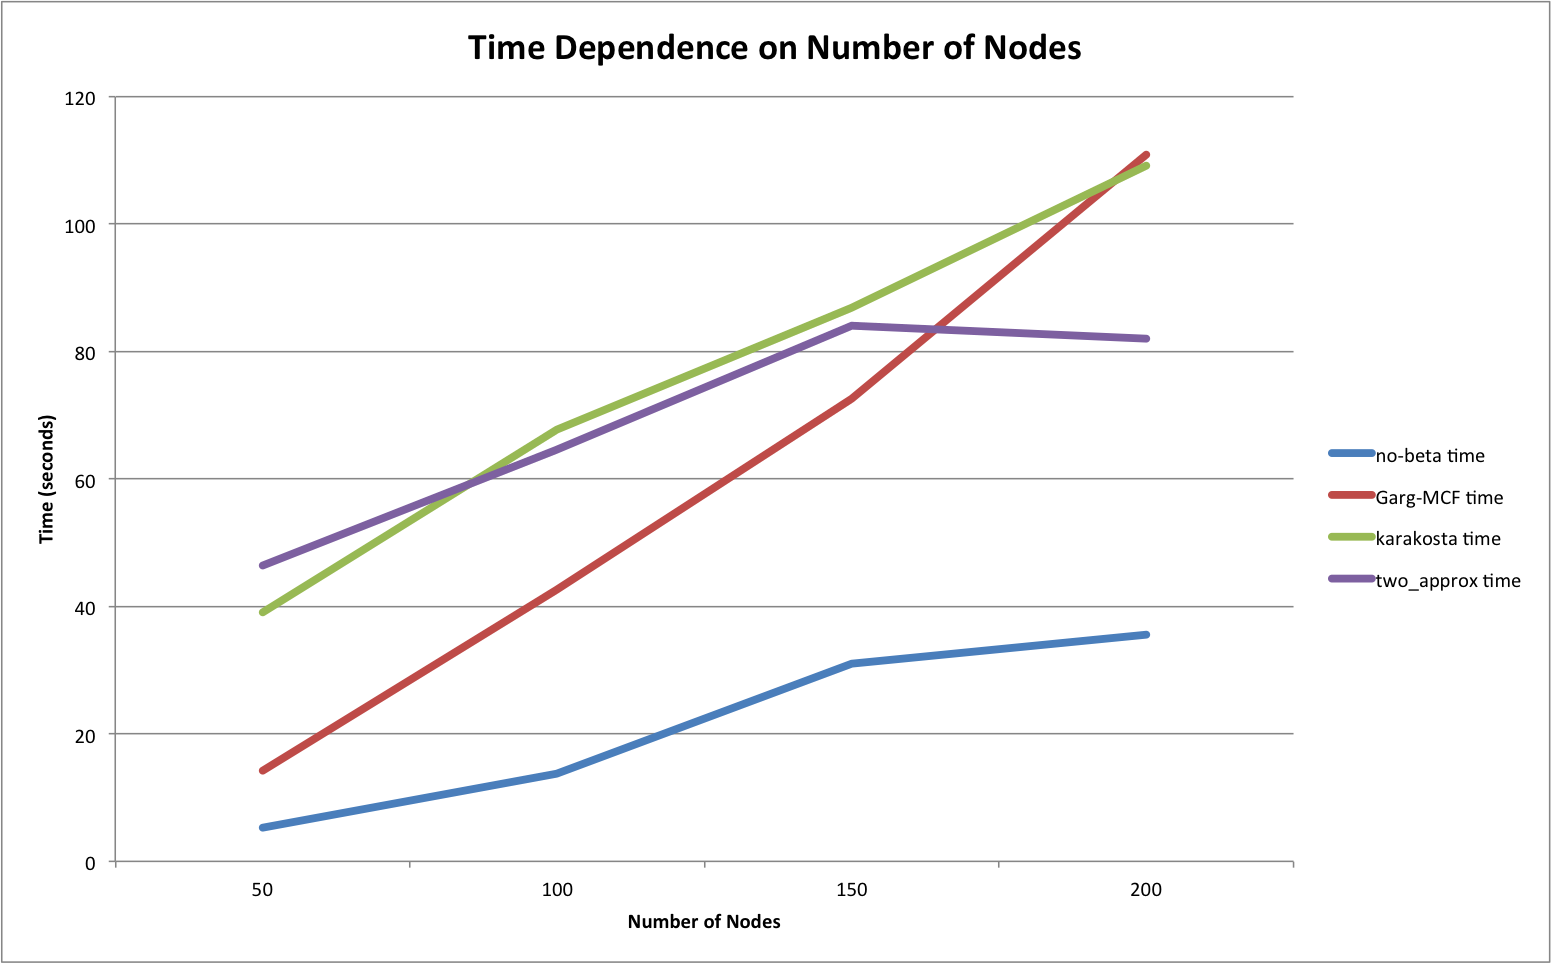
\includegraphics[width=0.8\textwidth]{figures/nodes-time.png}}
\caption{Plots of time in seconds versus number
  of nodes for all heuristics}
\end{center}
\end{figure*}

\begin{figure*}
\begin{center}
\mbox{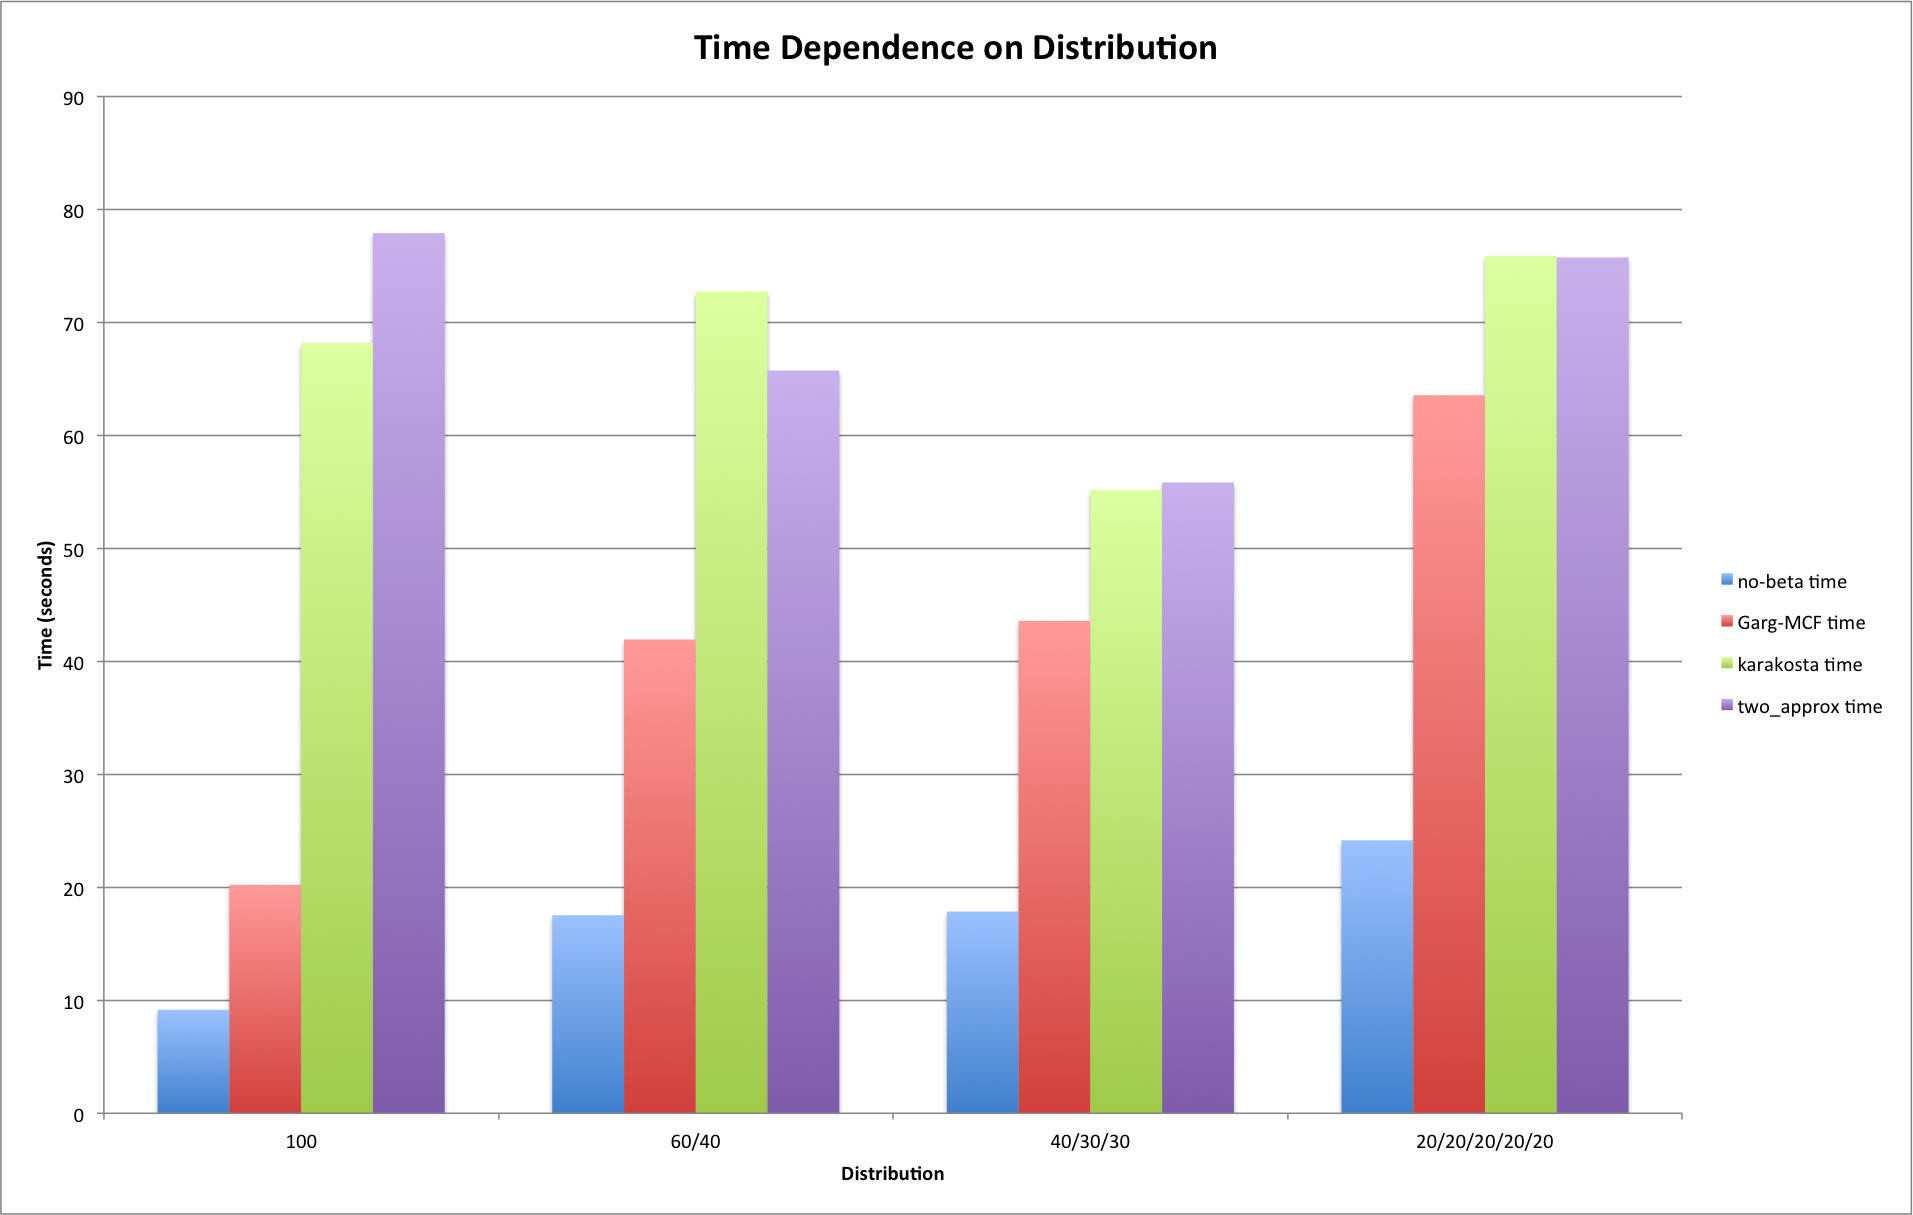
\includegraphics[width=0.8\textwidth]{figures/distribution-time.png}}
\caption{Plots of time in seconds versus distribution of commodities}
\end{center}
\end{figure*}



\end{document}
